\documentclass[aspectratio=169]{beamer}

\usepackage{xcolor}

\definecolor{codegray}{rgb}{0.85, 0.85, 0.85}

\usetheme{metropolis}
\setbeamertemplate{footline}{}
\setbeamertemplate{headline}{}

\title{Apache OpenWhisk}
\subtitle{Distributed Software Systems, 2024/25}
\author{Davide De Rosa}
\date{}

\begin{document}

\begin{frame}[plain]
    \titlepage
\end{frame}

%SLIDE 1: INTRODUCTION TO SERVERLESS COMPUTING
\section{Introduction to \\Serverless Computing}
\begin{frame}{Introduction to Serverless Computing}
\textbf{Serverless Computing} has transformed how we develop and deploy cloud applications. Traditional cloud computing required developers to manage virtual machines or containers, while \textbf{Serverless} eliminates this burden.\\
This model operates through \textbf{small}, \textbf{stateless functions} triggered by \textbf{events}, with the \textbf{cloud provider} managing backend infrastructure. Key benefits include:
\begin{itemize}
    \item \textbf{Autoscaling} to handle varying loads.
    \item A \textbf{pay-as-you-go} model, where costs align with actual function usage.
\end{itemize}
However, Serverless isn’t without its challenges. Cold starts, limited runtime languages, and debugging complexities still hinder its adoption.\\
Despite this, serverless computing has become integral to modern architectures, thanks to its simplicity and cost efficiency.
\end{frame}

%SLIDE 2: INTRODUCTION TO SERVERLESS COMPUTING
\begin{frame}{Introduction to Serverless Computing}
Over the past decade, cloud platform hosting has evolved significantly:
\begin{itemize}
    \item Initially, organizations purchased or rented physical servers to run applications, incurring costs for both the hardware and its maintenance.
    \item This shifted with the adoption of \textbf{virtualization}, which allowed a single physical server to function as multiple software-defined Virtual Machines (VMs), enhancing flexibility and resource utilization. \textbf{Containerization} emerged as a further refinement, combining aspects of virtualization with configuration management.
    \item The introduction of \textbf{Platform-as-a-Service} (\textbf{PaaS}) took abstraction further, freeing users from managing servers and deployment processes.
    \item The latest advancement, serverless computing, builds on \textit{PaaS} by enabling deployment of small code fragments that can autonomously scale, supporting the creation of self- scaling applications.
\end{itemize}
\end{frame}

%SLIDE 3: SERVERLESS ARCHITECTURE
\section{Serverless Architecture}
\begin{frame}{Serverless Architecture}
At its core, Serverless Computing revolves around simplicity and efficiency. Functions run in isolated containers, with each triggered by specific events like HTTP requests or database updates.
The process begins when an event triggers the platform:
\begin{itemize}
    \item An \textbf{event queue} receives the trigger and informs a dispatcher.
    \item The \textbf{dispatcher} assigns the function to a \textbf{worker node}.
    \item If a \textbf{worker} is free, it executes the function. Otherwise, the request is queued.
\end{itemize}
A load balancer ensures smooth operations, though challenges like resource contention and cold starts remain. To address this, providers pre-warm containers, minimizing latency during new invocations.    
\end{frame}

%SLIDE 4: SERVERLESS ARCHITECTURE
\begin{frame}{Serverless Architecture}
\centering
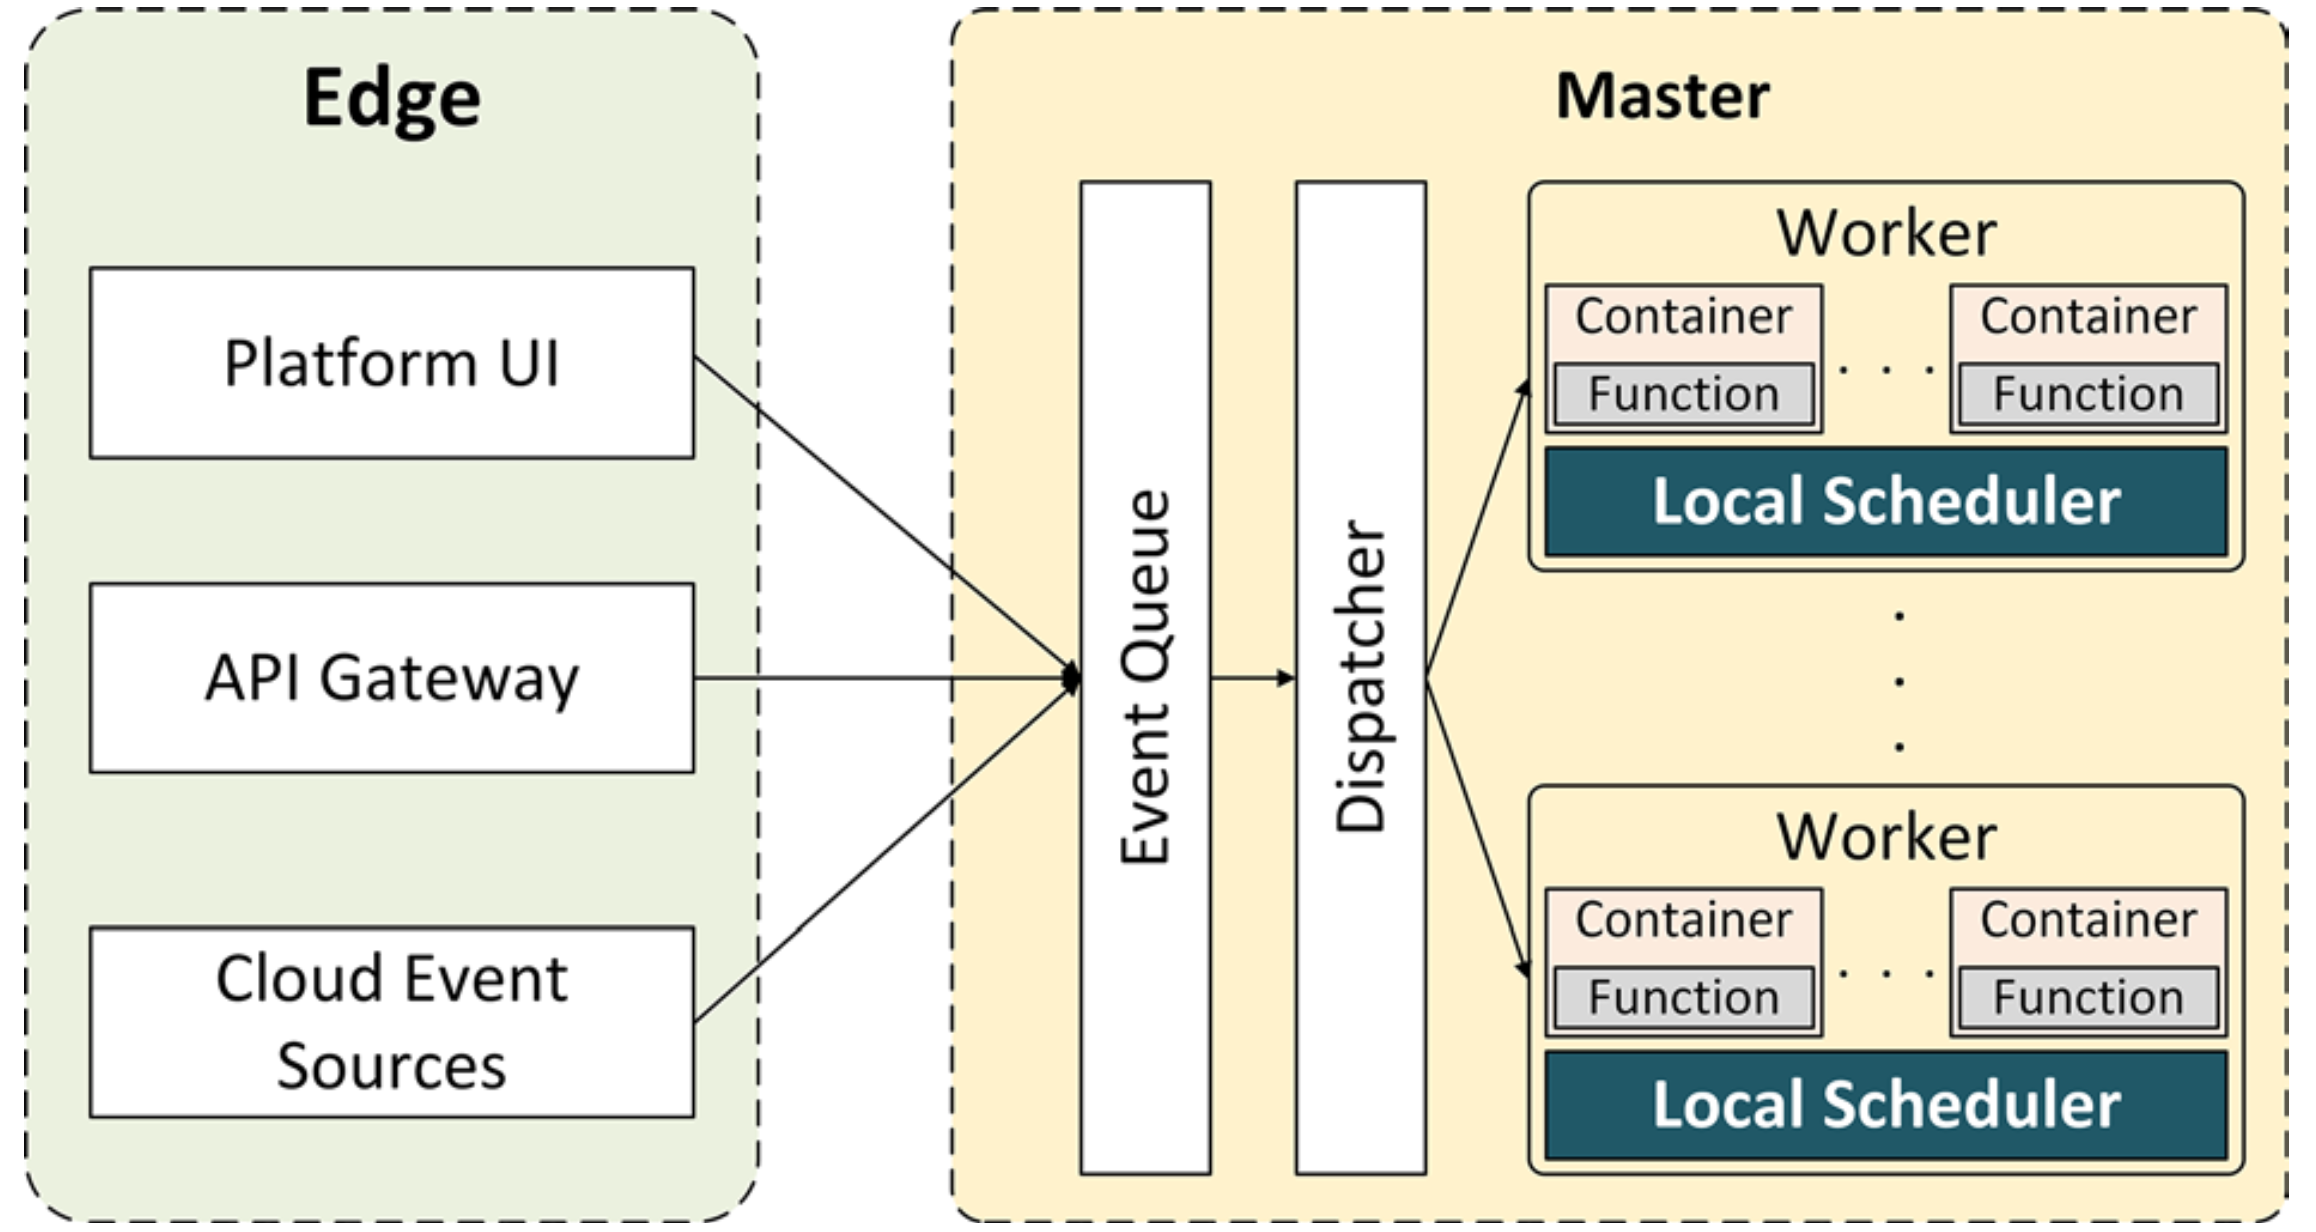
\includegraphics[width=0.8\textwidth]{img/arch.png}
\end{frame}

%SLIDE 5: APACHE OPENWHISK
\section{Apache Openwhisk}
\begin{frame}{Apache Openwhisk}
\textbf{Apache Openwhisk} is \textbf{IBM}’s \textbf{open-source} serverless platform. It competes with giants like \textit{AWS Lambda} and \textit{Google Cloud Functions} by offering flexibility and openness. Developers use Openwhisk to build applications requiring \textit{real-time processing}, \textit{IoT data handling}, or \textit{serverless APIs}.\\
Its design is \textbf{event-driven}, and its programming model is built around three elements:
\begin{itemize}
    \item \textbf{Actions}: Stateless functions that process events.
    \item \textbf{Triggers}: Events that activate functions.
    \item \textbf{Rules}: Bindings connecting triggers to actions.
\end{itemize}
What sets Openwhisk apart is its adaptability. It supports deployment on platforms like \textit{Kubernetes} and \textit{OpenShift}, and its CLI tool makes it accessible across operating systems.
\end{frame}

%SLIDE 6: APACHE OPENWHISK
\begin{frame}{Apache Openwhisk}
\centering
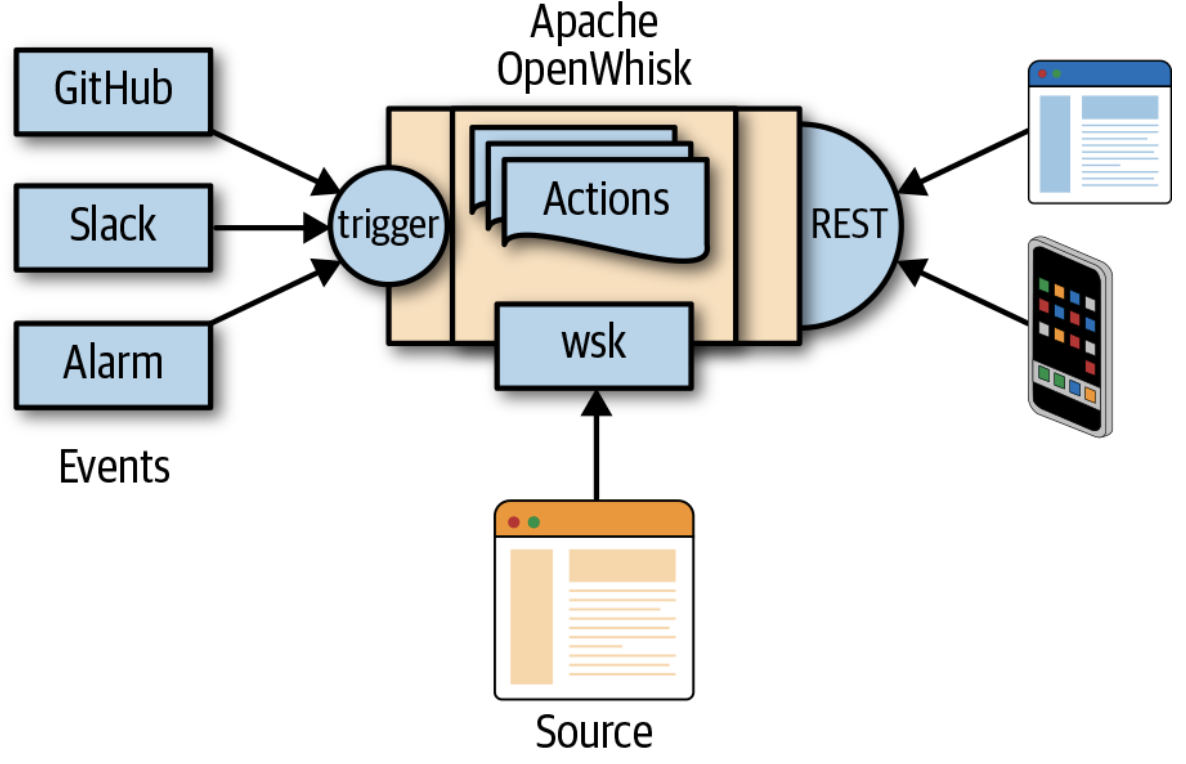
\includegraphics[width=0.75\textwidth]{img/ow_works.png}
\end{frame}

%SLIDE 7: APACHE OPENWHISK
\begin{frame}{Apache Openwhisk Key Features}
\begin{itemize}
    \item \textbf{Deploys Anywhere}: with its container-based architecture, Openwhisk offers versatile deployment options, supporting local setups and cloud infrastructures.
    \item \textbf{Supports Any Programming Language}: Openwhisk is compatible with a wide range of programming languages. For unsupported platforms or languages, users can easily create and customize executables using Docker.
    \item \textbf{Integration Support}: Openwhisk enables easy integration of developed Actions with popular services through pre-built packages.
    \item \textbf{Rich Function Composition}: functions written in multiple programming languages can be packaged with Docker for flexible invocation options, including synchronous, asynchronous, or scheduled execution.
    \item \textbf{Scalability and Resource Optimization}: Openwhisk allows Actions to scale instantly. Resources scale automatically to match demand, pausing when idle, so users only pay for actual usage with no costs for unused resources.
\end{itemize}
\end{frame}

%SLIDE 8: APACHE OPENWHISK MAIN ARCHITECTURAL DRIVERS
\section{Apache Openwhisk \\Main Architectural Drivers}
\begin{frame}{Apache Openwhisk Main Architectural Drivers}
The success of Apache Openwhisk lies in its architectural foundations, tailored to meet the demands of Serverless Computing:
\begin{itemize}
    \item \textbf{Scalability and Elasticity}: stateless functions scale instantly to meet demand. Openwhisk leverages containerized isolation for rapid provisioning.
    \item \textbf{Low Latency}: pre-warming containers addresses the infamous cold start issue.
    \item \textbf{Fault Tolerance}: using \textit{Apache Kafka} as a messaging backbone ensures reliable event handling, even in distributed setups.
    \item \textbf{Extensibility}: Openwhisk’s modular architecture lets developers customize runtimes, add integrations, or tailor deployments for hybrid clouds.
    \item \textbf{Security}: containers provide isolation, while role-based access control and encrypted communications strengthen protection.
\end{itemize}
By addressing these factors, Openwhisk aligns with enterprise needs while maintaining its open-source ethos.
\end{frame}

%SLIDE 9: APACHE OPENWHISK ARCHITECTURE
\section{Apache Openwhisk Architecture}
\begin{frame}{Apache Openwhisk Architecture}
Openwhisk’s architecture consists of two primary components: the \textbf{Controller} and the \textbf{Invoker}, built on \textbf{Nginx}, \textbf{Kafka}, \textbf{Docker}, and \textbf{CouchDB}.\vspace{14pt}\\
Together, these components enable Openwhisk to function as a \textbf{serverless event-driven} programming service.\vspace{14pt}\\
Openwhisk offers a \textit{RESTful API} that allows users to submit functions and retrieve execution results.
\end{frame}

%SLIDE 10: APACHE OPENWHISK ARCHITECTURE
\begin{frame}{Apache Openwhisk Architecture}
\centering
\includegraphics[width=0.6\textwidth]{img/ow_arch.png}
\end{frame}

%SLIDE 11: APACHE OPENWHISK ARCHITECTURE
\begin{frame}{Apache Openwhisk Architecture}
\textbf{Nginx} routes incoming requests to the \textit{Controller}, which handles authentication, retrieves the requested functions from the \textbf{CouchDB} database, and directs them to the \textit{Invokers} acting as a \textit{Load Balancer}.\vspace{14pt}\\
\textbf{Kafka}, a high-performance message distribution system, facilitates communication between the \textit{Controller} and the \textit{Invokers}.\vspace{14pt}\\
The \textit{Invokers}, distributed across multiple machines and responsible for hosting serverless function containers, execute function calls by allocating resources within \textbf{Docker} containers and assigning a container to each function invocation. Essentially, \textit{Invokers} serve as the worker nodes in Openwhisk.
\end{frame}

%SLIDE 12: APACHE OPENWHISK ARCHITECTURE
\begin{frame}{Apache Openwhisk Architecture}
Each \textit{Invoker} has an in-memory queue to manage function requests when resources are temporarily unavailable. Once resources are freed, functions are dequeued and executed in a \textbf{First Come First Serve} (\textbf{FCFS}) order.\vspace{14pt}\\
All \textit{Invokers} use the same instructions embedded in the \textit{Invoker component’s source code} (written in \textit{Scala}), ensuring uniform operation across all \textit{Invokers}.\vspace{14pt}\\
Users can register on the platform to upload their functions, specifying only the memory required for each function’s execution.
\end{frame}

%SLIDE 13: COMPETING SOLUTIONS
\section{Competing solutions}
\begin{frame}{Competing solutions}
\begin{itemize}
    \item \textbf{AWS Lambda}
    \begin{itemize}
        \item \textbf{Strength}: deep integration with AWS services.
        \item \textbf{Weakness}: vendor lock-in.
        \item \textbf{Comparison}: Lambda excels in AWS ecosystems, while Openwhisk’s open-source model appeals to those avoiding lock-in.
    \end{itemize}
    \item \textbf{Google Cloud Functions}
    \begin{itemize}
        \item \textbf{Strength}: low latency and tight GCP integration.
        \item \textbf{Weakness}: limited multi-cloud deployment.
        \item \textbf{Comparison}: Openwhisk offers more deployment flexibility.
    \end{itemize}
    \item \textbf{Azure Functions}
    \begin{itemize}
        \item \textbf{Strength}: strong .NET support.
        \item \textbf{Weakness}: constrained by Azure’s ecosystem.
        \item \textbf{Comparison}: Openwhisk’s language agnosticism and hybrid deployment edge out Azure for broader needs.
    \end{itemize}
\end{itemize}
\end{frame}

%SLIDE 14: IMPLEMENTATION
\section{Implementation}
\begin{frame}{Implementation}
Using the \textit{OpenServerless CLI} (\textbf{ops}), I managed to get everything up and running on the virtual machine. I then wrote a really simple \textbf{Python} script, which returns an \textit{Hello World} message:\vspace{14pt}\\
\centering
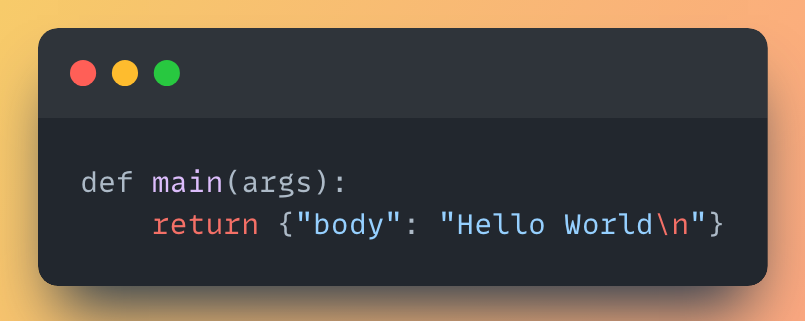
\includegraphics[width=0.7\textwidth]{img/code_snippet.png}
\end{frame}

%SLIDE 15: IMPLEMENTATION
\begin{frame}{Implementation}
Using the \vspace{-15pt}
\begin{center}
    \colorbox{codegray}{\texttt{ops package create test dss}}\vspace{-5pt}
\end{center} 
command, I created a test package where actions can be stored.\vspace{-5pt}
\begin{center}
    \colorbox{codegray}{\texttt{ops action create test dss/greet script.py --web true}}\vspace{-5pt} 
\end{center}
is going to create the action related to the Python script.\\
Using the \textbf{–web} flag with a value of \textbf{true} or \textbf{yes} allows an action to be accessible via \textbf{REST} interface without the need for credentials.
To get the URL related to the action, the \vspace{-15pt}
\begin{center}
    \colorbox{codegray}{\texttt{ops action get test dss/greet --url}}\vspace{-5pt}
\end{center}
command is used. This returns the action HTTP endpoint, ready to be called and tested.
\end{frame}

%SLIDE 16: IMPLEMENTATION
\begin{frame}{Implementation}
An example of this whole execution of commands can be:\vspace{14pt}\\
\centering
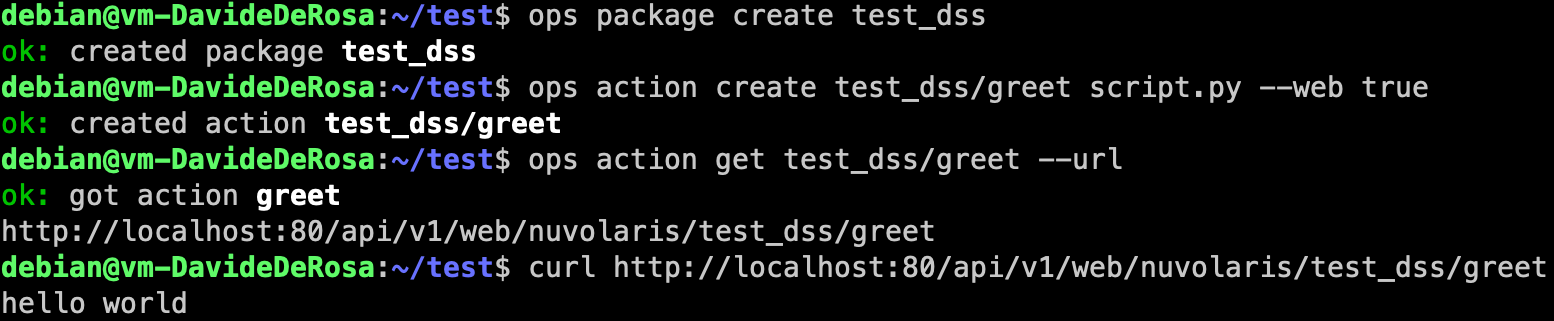
\includegraphics[width=1\textwidth]{img/demo.png}
\end{frame}

%SLIDE 17: IMPLEMENTATION
\begin{frame}{Implementation}
Heartfelt thanks go to \textit{Michele Sciabarrà} and his team, for real-time support while debugging the various problems encountered.\vspace{14pt}\\
\begin{minipage}{0.55\textwidth}
    Also, a big thank you to the \textbf{ADM team} – \\
    especially \textit{Emanuele Grasso}. Thanks to his support, I was provided with a virtual machine that met the requirements of OpenServerless and allowed me to perform all the necessary tests.\vspace{6pt}\\
    Their work goes beyond this, providing a very useful service for all students in the Computer Science department and beyond.
\end{minipage}
\hfill
\begin{minipage}{0.4\textwidth}
    \centering
    
\includegraphics[width=0.8\textwidth]{img/adm_logo.png}
\end{minipage}
\end{frame}

\section*{References}
\begin{frame}{References}
    \begin{itemize}
        \item Etas: predictive scheduling of functions on worker nodes of apache openwhisk platform (Banaei, Ali and Sharifi, Mohsen), 2022
        \item Evaluating apache openwhisk-faas, Quevedo (Sebasti{\'a}n and Merch{\'a}n, Freddy and Rivadeneira, Rafael and Dominguez, Federico X), 2019
        \item Crypto currencies prices tracking microservices using apache OpenWhisk (Huy, Lam Phuoc and Saifullah, Saifullah and Sahillioglu, Marcel and Baun, Christian), 2021 
        \item Open-source serverless architectures: an evaluation of apache openwhisk (Djemame, Karim and Parker, Matthew and Datsev, Daniel), 2020
        \item LEARNING APACHE OPENWHISK: developing open serverless solutions (Sciabarr{\`a}, Michele), 2019
    \end{itemize}
\end{frame}
\end{document}